%texexptitled======================================================================
% lab1-gcd
%-----------------------------------------------------------------------
%

\documentclass[11pt]{article}

% Package includes

\usepackage{graphicx}
\usepackage{color}
\usepackage{comment}
\usepackage{multirow}
\usepackage{askmaps}
\usepackage{amssymb}
\usepackage{amsmath}
\usepackage{tikz}
\usepackage{circuitikzgit}
\usetikzlibrary{arrows, positioning, shapes.geometric, circuits.logic.US}
\tikzstyle{line}=[draw]
\tikzstyle{arrow}=[draw, -latex]

% Wrap long URLs with hyphens
\PassOptionsToPackage{hyphens}{url}\usepackage{hyperref}
\usepackage{pdftexcmds}
\usepackage{upquote}
\usepackage{textcomp}
\usepackage{minted}
\usepackage[listings]{tcolorbox}
\usepackage{enumerate}
\usepackage{enumitem}
\usepackage{mathtools}
\DeclarePairedDelimiter{\ceil}{\Big\lceil}{\Big\rceil}

\tcbset{
texexp/.style={colframe=black, colback=lightgray!15,
         coltitle=white,
         fonttitle=\small\sffamily\bfseries, fontupper=\small, fontlower=\small},
     example/.style 2 args={texexp,
title={Question \thetcbcounter: #1},label={#2}},
}

\newtcolorbox{texexp}[1]{texexp}
\newtcolorbox[auto counter]{texexptitled}[3][]{%
example={#2}{#3},#1}

\setlength{\topmargin}{-0.5in}
\setlength{\textheight}{9in}
\setlength{\oddsidemargin}{0in}
\setlength{\evensidemargin}{0in}
\setlength{\textwidth}{6.5in}

% Useful macros

\newcommand{\note}[1]{{\bf [ NOTE: #1 ]}}
\newcommand{\fixme}[1]{{\bf [ FIXME: #1 ]}}
\newcommand{\wunits}[2]{\mbox{#1\,#2}}
\newcommand{\um}{\mbox{$\mu$m}}
\newcommand{\xum}[1]{\wunits{#1}{\um}}
\newcommand{\by}[2]{\mbox{#1$\times$#2}}
\newcommand{\byby}[3]{\mbox{#1$\times$#2$\times$#3}}


\newenvironment{tightlist}
{\begin{itemize}
 \setlength{\parsep}{0pt}
 \setlength{\itemsep}{-2pt}}
{\end{itemize}}

\newenvironment{titledtightlist}[1]
{\noindent
 ~~\textbf{#1}
 \begin{itemize}
 \setlength{\parsep}{0pt}
 \setlength{\itemsep}{-2pt}}
{\end{itemize}}

% Change spacing before and after section headers

\makeatletter
\renewcommand{\section}
{\@startsection {section}{1}{0pt}
 {-2ex}
 {1ex}
 {\bfseries\Large}}
\makeatother

\makeatletter
\renewcommand{\subsection}
{\@startsection {subsection}{1}{0pt}
 {-1ex}
 {0.5ex}
 {\bfseries\normalsize}}
\makeatother

% Reduce likelihood of a single line at the top/bottom of page

\clubpenalty=2000
\widowpenalty=2000

% Other commands and parameters

\pagestyle{myheadings}
\setlength{\parindent}{0in}
\setlength{\parskip}{10pt}

% Commands for register format figures.

\newcommand{\instbit}[1]{\mbox{\scriptsize #1}}
\newcommand{\instbitrange}[2]{\instbit{#1} \hfill \instbit{#2}}

\newif\ifsolution

\if\issolution1
\newenvironment{solution}
    {\color{red}}
    {\color{black}}
\solutiontrue
\else
\excludecomment{solution}
\solutionfalse
\fi


\graphicspath{{./figs/}}


%-----------------------------------------------------------------------
% Document
%-----------------------------------------------------------------------

\begin{document}
\def\PYZsq{\textquotesingle}


\newcommand{\headertext}{EE142 Problem Set 5}

\title{\vspace{-0.4in}\Large \bf \headertext \vspace{-0.1in}}
\author{Vighnesh Iyer}

\date{\today}
\maketitle

\markboth{\headertext}{\headertext}
\thispagestyle{empty}

\section*{Problem 1}
{\color{blue}Find $y$ for the following normalized impedance on Smith Chart.}

The straightforward procedure is to plot $z_L$ on the impedance Smith Chart, and then look at what constant admittance and constant suspectance curves cross over the point in the admittance smith chart.

But, we can also plot $z_L$ on the impedance smith chart, then rotate the point by $\pi$ degrees along the constant SWR circle, and then read off the admittance by looking at the constant resistance and reactance curves.

I'm going to use the second technique; annotated charts aren't included in this document, but I'll compare the chart result I get to the exact calculation.
\begin{enumerate}[label=(\alph*)]
    \item $z_L = 1.4 + 2j$
    \begin{align*}
        y_L = \frac{1}{z_L} = \frac{1}{\alpha + \beta j} = \frac{\alpha - \beta j}{\alpha^2 + \beta^2} &= 0.234899 -0.33557 j \\
        y_{L,chart} &= 0.22 - 0.32j
    \end{align*}

    \item $z_L = 0.5 + 0.9j$
    \begin{align*}
        y_L &= 0.471698 - 0.849 j \\
        y_{L,chart} &= 0.45 - 0.85j
    \end{align*}

    \item $z_L = 1.6 - 0.3j$
    \begin{align*}
        y_L &= 0.60377 + 0.1132j \\
        y_{L,chart} &= 0.6 + 0.12j
    \end{align*}
\end{enumerate}

\section*{Problem 2}
{\color{blue}Use the Smith Chart. Also use equations for lumped component matching to check.}
\begin{enumerate}[label=(\alph*)]
    \item Match $Z_L = 70 + 100j \Omega$ to 50 Ohm with lumped components.

    Let's clear up some things:
    \begin{align*}
        Z_C &= \frac{1}{j \omega C} & X_C &= \Im{Z_C} = - \frac{1}{\omega C} \\
        Z_L &= j \omega L & X_L &= \Im{Z_L} = \omega L \\
        \text{To find } C &= \frac{1}{\omega X_c} \\
        \text{To find } L &= \frac{X_L}{\omega} \\
        \text{where: } \omega &= 2 \pi f
    \end{align*}

    The load is complex, so we have to resonant out the load's complex impedance so only a real part is seen before solving using the L network method.
    \begin{figure}[H]
        \begin{center}
            \begin{circuitikz}
                \draw (0,0) to[generic] (0,-2);
                \draw (-2,0) to[generic] (0,0);
                \draw (-2,0) to[generic] (-2,-2);
                \draw (-4,0) to[generic] (-2,-0);
                \draw (-4.25,0) to[short, o-] (-4,0);
                \draw (0,-2) node[ground] (ground) {};
                \draw (-2,-2) node[ground] (ground1) {};
                \node[draw=none] at (1.25, -1) {$70 + 100j$};
                \node[draw=none] at (-1, 0.5) {$-100j$};
                \node[draw=none] at (-1.5, -1) {$L$};
                \node[draw=none] at (-3, 0.5) {$C$};
            \end{circuitikz}
        \end{center}
    \end{figure}

    Now, the L-network will see a purely real $70\Omega$ impedance with which we can use the regular matching equations.
    \begin{align*}
        R_S &= 50 \\
        R_L &= 70 \\
        R_{hi} &= max(R_S, R_L) = 70 \\
        R_{lo} &= min(R_S, R_L) = 50 \\
        \text{Boosting factor: } m &= \frac{R_{hi}}{R_{lo}} = 1.4 \\
        Q &= \sqrt{m-1} = 0.632 \\
        \text{Dropping resistance so, } X_p &= \frac{R_L}{Q} = 110.76 \\
        X_p' &= \frac{X_p}{1 + Q^{-2}} = 31.613 \\
        X_s &= -X_p' = -31.613
    \end{align*}

    We arrive at the capacitor reactance of $-79.15j$ and the inductor reactance of $110.76j$.
    The circuit is simulated in ADS to match at 1 Ghz with component values $C = 5.0344$ pF, $L = 17.6$ nH, and $C_{res} = 1.59$ pF.
    S-parameter simulation verifies that the source and load are perfectly matched at 1 Ghz with $S_{21} = 0 dB$.

    The same calculation can be performed using the smith chart.
    \begin{align*}
        Z_{L,norm} &= 1.4 + 2j \\
        Z_{L,real} &= 1.4 \\
        X_p = (1/0.45)j \cdot 50 &= 111.1j \\
        X_s = -0.62 \cdot 50 &= -31j
    \end{align*}

    The values calculated using the Smith Chart are very close to the values from the equations.

    \item Match $Z_L = 70 + 100j \Omega$ to 50 Ohm using transmission lines.
    \item Match $Z_L = 160 - 30j \Omega$ to 100 Ohm using lumped circuits.

    Assume a resonating inductor with reactance $30j$ to make the load purely real.
    \begin{align*}
        R_S &= 100 \\
        R_L &= 160 \\
        R_{hi} &= max(R_S, R_L) = 160 \\
        R_{lo} &= min(R_S, R_L) = 100 \\
        \text{Boosting factor: } m &= \frac{R_{hi}}{R_{lo}} = 1.6 \\
        Q &= \sqrt{m-1} = 0.775 \\
        \text{Dropping resistance so, } X_p &= \frac{R_L}{Q} = 206.452 \\
        X_p' &= \frac{X_p}{1 + Q^{-2}} = 77.47 \\
        X_s &= -X_p' = -77.47
    \end{align*}

    We simulate in ADS with $L_{res} = 4.77$ nH, $L = 32.858$ nH, $C = 2.05$ pF.
    The simulation shows that these values give a perfect match at 1 Ghz. This match appears more broadband than the one in part a). The Smith Chart again gives very similar values.

    \item Match $Z_L = 160-30j \Omega$ to 100 Ohm using transmission lines.

    \item Match $Z_L = 25 + 90j \Omega$ to 50 Ohm using lumped circuits.
    Assume a resonating capacitor with reactance $-90j$ to make the load purely real.
    \begin{align*}
        R_S &= 50 \\
        R_L &= 25 \\
        R_{hi} &= max(R_S, R_L) = 50 \\
        R_{lo} &= min(R_S, R_L) = 25 \\
        \text{Boosting factor: } m &= \frac{R_{hi}}{R_{lo}} = 2.0 \\
        Q &= \sqrt{m-1} = 1.0 \\
        \text{Boosting resistance so, } X_s &= Q \cdot R_L = 25 \\
        X_s' &= X_s(1 + Q^{-2}) = 50 \\
        X_p &= -X_s' = -50
    \end{align*}

    We simulate in ADS with $C_{res} = 1.768$ pF, $C = 3.183$ pF, $L = 3.98$ nH. The results confirm a perfect match at 1 Ghz.

    \item Match $Z_L = 25 + 90j \Omega$ to 50 Ohm using transmission lines.
\end{enumerate}

\section*{Problem 3}

\begin{enumerate}[label=(\alph*)]
    \item {\color{blue}Design a $\Pi$ matching network between a 1000$\Omega$ load impedance and a $50 \Omega$ source impedance at 1 Ghz. The inductor and capacitor quality factors are 20. The target bandwidth for $|S_{11}| < -10$ dB is 5\%. Calculate the insertion loss and verify your design using ADS. Check if $|S_{11}|^2 + |S_{21}|^2 = 1$ holds.}

    Let's first analyze an L-network to see if it can fit our design requirements.

    \begin{align*}
        Q_{cap} &= Q_{ind} = 20 \\
        m = \frac{R_{hi}}{R_{lo}} = 20 \rightarrow Q &= \sqrt{m-1} \approx 4.359 \\
        Q_{total,L-network} &= \frac{Q}{2} \approx 2.2 \\
        S_{11} \text{ -10 dB BW} &\approx \frac{1}{3 \cdot Q_{total}} = 15\% \\
        \text{Insertion Loss} &= \frac{1}{1 + \frac{Q}{Q_{cap}} + \frac{Q}{Q_{ind}}} = 0.694
    \end{align*}

    The bandwidth of the L-network is too high and isn't selective enough for our requirements.
    The bandwidth is set (approximately) by the circuit Q and so we need to use a $\Pi$ network so $Q$ doesn't depend on $m$.

    \begin{align*}
        \frac{1}{3 \cdot Q_{tot}} \approx 0.05 \rightarrow Q_{tot} &\geq 6 \\
        Q_1 &= \sqrt{\frac{R_L}{R_i} - 1} \\
        Q_2 &= \sqrt{\frac{R_S}{R_i} - 1} \\
        Q_{tot} &= \frac{Q_1 + Q_2}{2} \\
        R_i &\leq 8.108
    \end{align*}

    We find that the intermediate resistance should be less than 8.108 $\Omega$ to keep the bandwidth below 5\%. We will design for $R_i = 5 \Omega$.

    Here are all the derived parameters:

    \begin{center}
    \begin{tabular}{l | l | l |}
        & L-network 1 & L-network 2 \\ \hline
        m & 200 & 10 \\ \hline
        Q & 14.11 & 3 \\ \hline
        $X_p$ & 70.888 & 16.666 \\ \hline
        $X_s$ & 70.534 & 15.0 \\ \hline
        $C$ & 2.245 pF & 9.549 pF \\ \hline
        $L$ & 11.2 nH & 1.39 nH \\ \hline
    \end{tabular}
    \end{center}

    assuming capacitors are placed in parallel and inductors in series. $Q_{tot}$ is around 8.5.

    \begin{figure}[H]
        \begin{center}
            \begin{circuitikz}
                \draw (0,0) to[vsourcesin] (0,2)
                    to[R, l=$50 \Omega$] (2,2)
                    to[generic, l=$L_1 + L_2$] (4,2)
                    to[generic, l=$C_1$] (4,0);
                \draw (4,2) to[short] (6,2)
                    to[R, l=$1000 \Omega$] (6,0);
                \draw (2,2) to[generic,l=$C_2$] (2,0);

                \draw (0,0) node[ground] (ground1) {};
                \draw (2,0) node[ground] (ground1) {};
                \draw (4,0) node[ground] (ground1) {};
                \draw (6,0) node[ground] (ground1) {};
            \end{circuitikz}
        \end{center}
    \end{figure}

    \begin{figure}[H]
        \centering 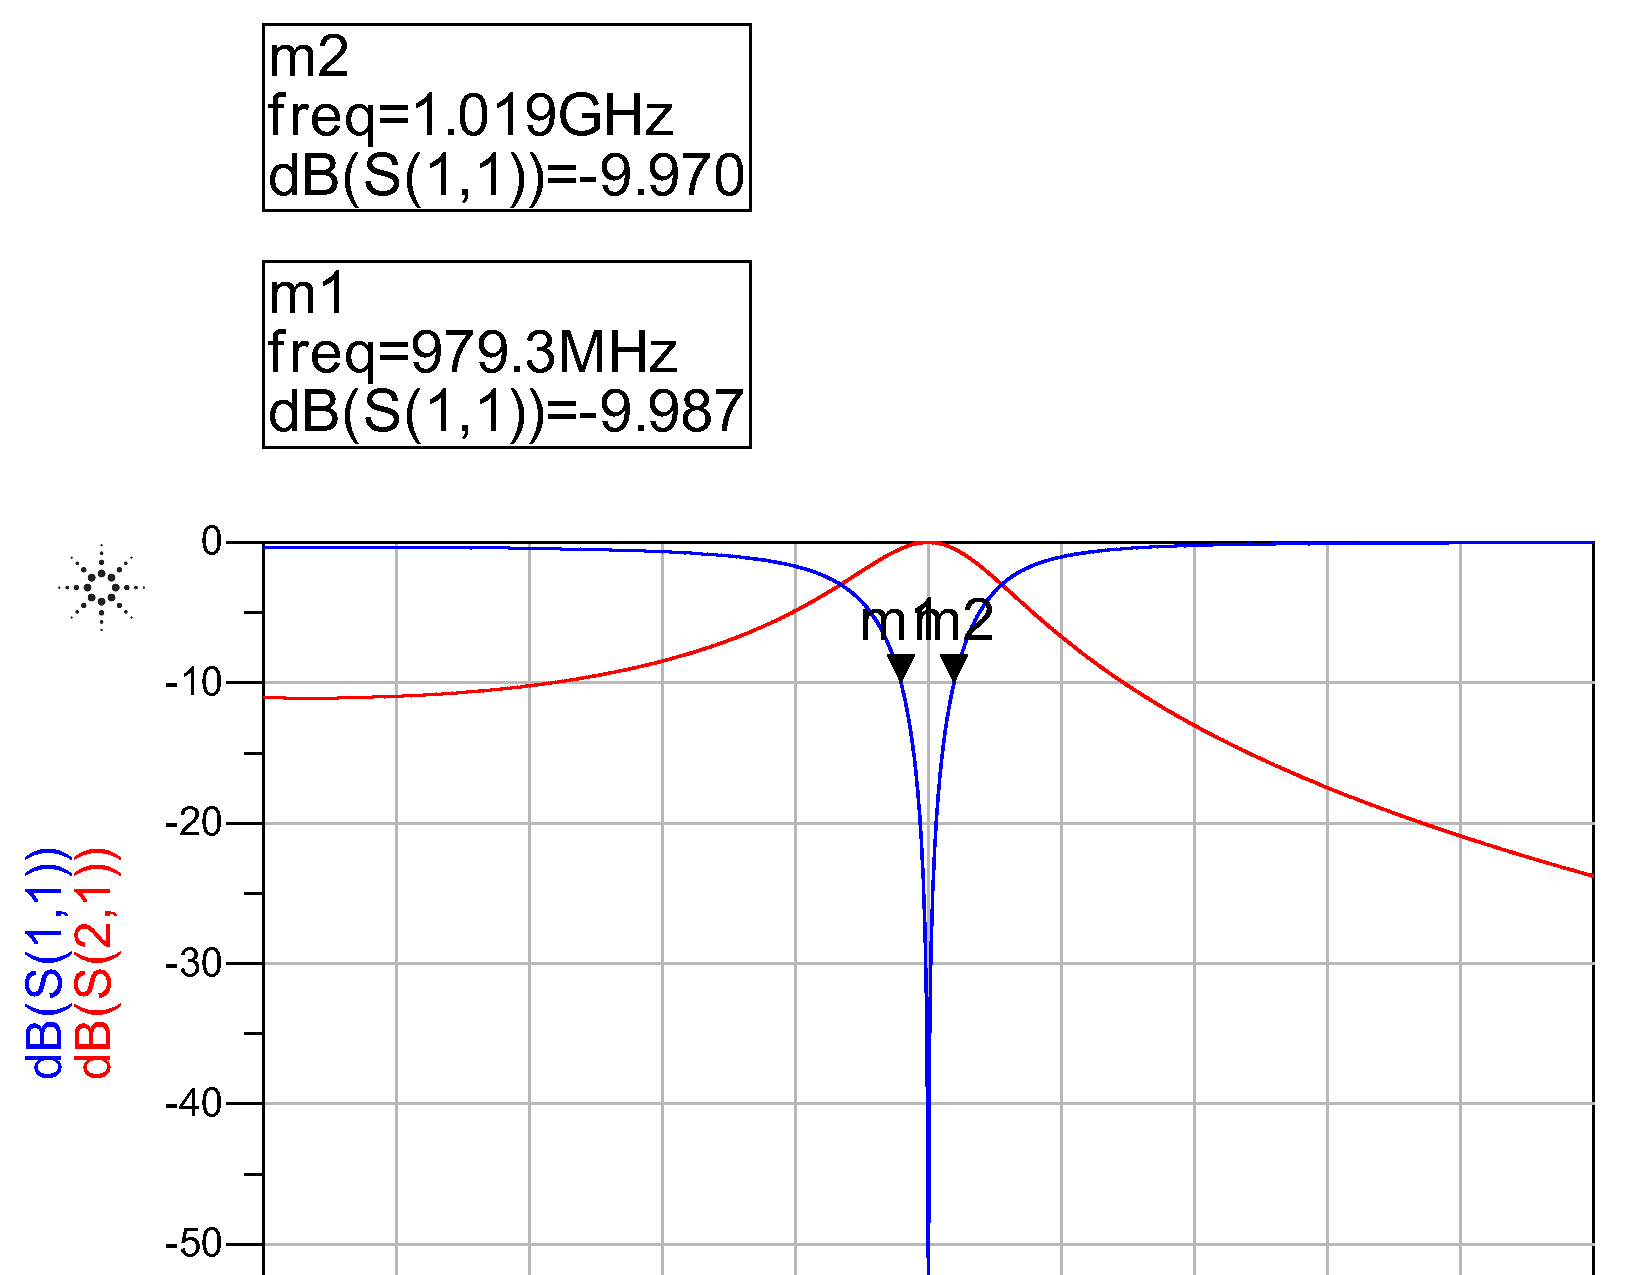
\includegraphics[width=\textwidth-4cm]{problem3a_bandwidth.pdf}
        \caption{Simulation with lossless components}
    \end{figure}

    We run a simulation and find that for lossless components, the bandwidth of $S_{11}$ down to -10 dB is 39.7 Mhz, which is within our 50 Mhz design spec.

    \begin{figure}[H]
        \centering 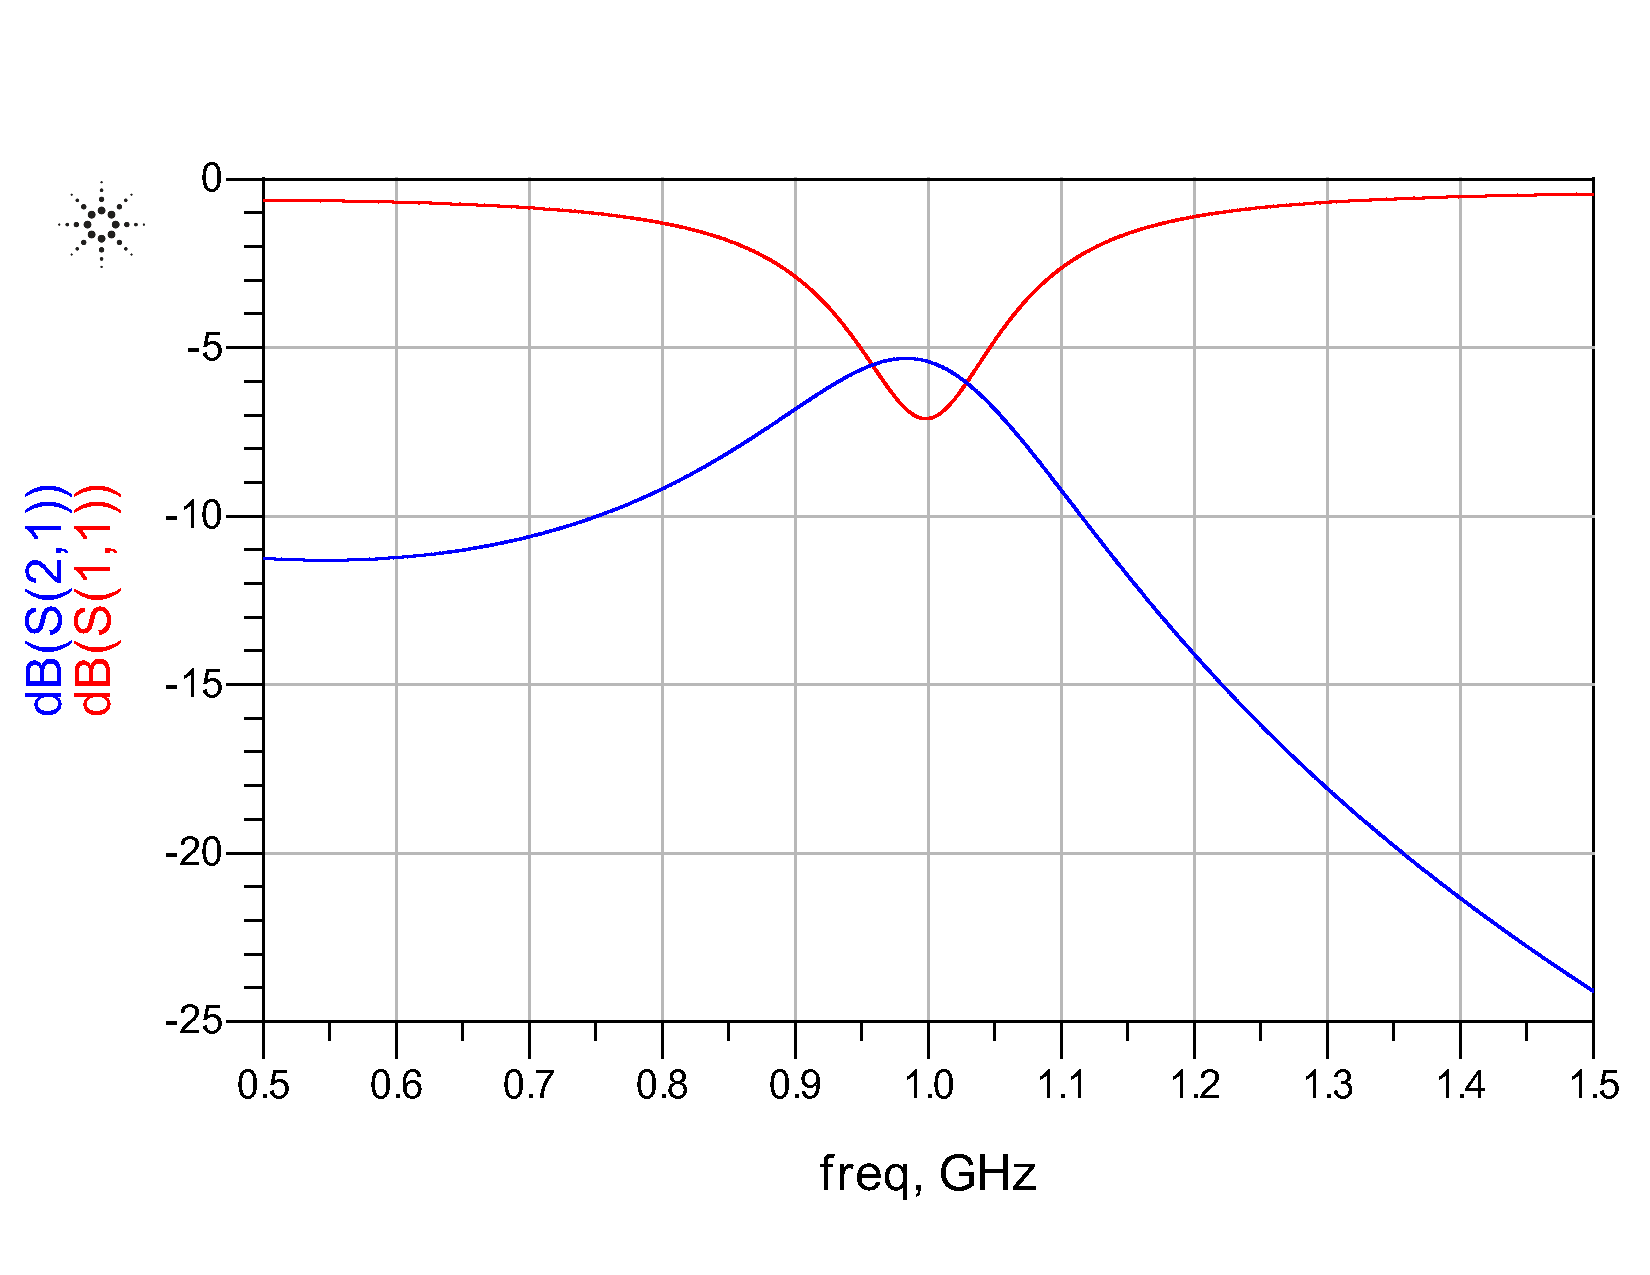
\includegraphics[width=\textwidth-4cm]{problem3a_finite_q.pdf}
        \caption{Simulation with finite Q}
    \end{figure}
    When adding finite Q components, the bandwidth isn't very different, but the insertion loss at 1 Ghz becomes significant.
    However the $S_{11}$ -10dB bandwidth becomes infinite/zero since $S_{11}$ never dips below -10dB.
    It is possible that the Q of these components isn't sufficient to achieve -10dB input selectivity.
    It's also possible that my design isn't optimized sufficiently.

    \begin{figure}[H]
        \centering 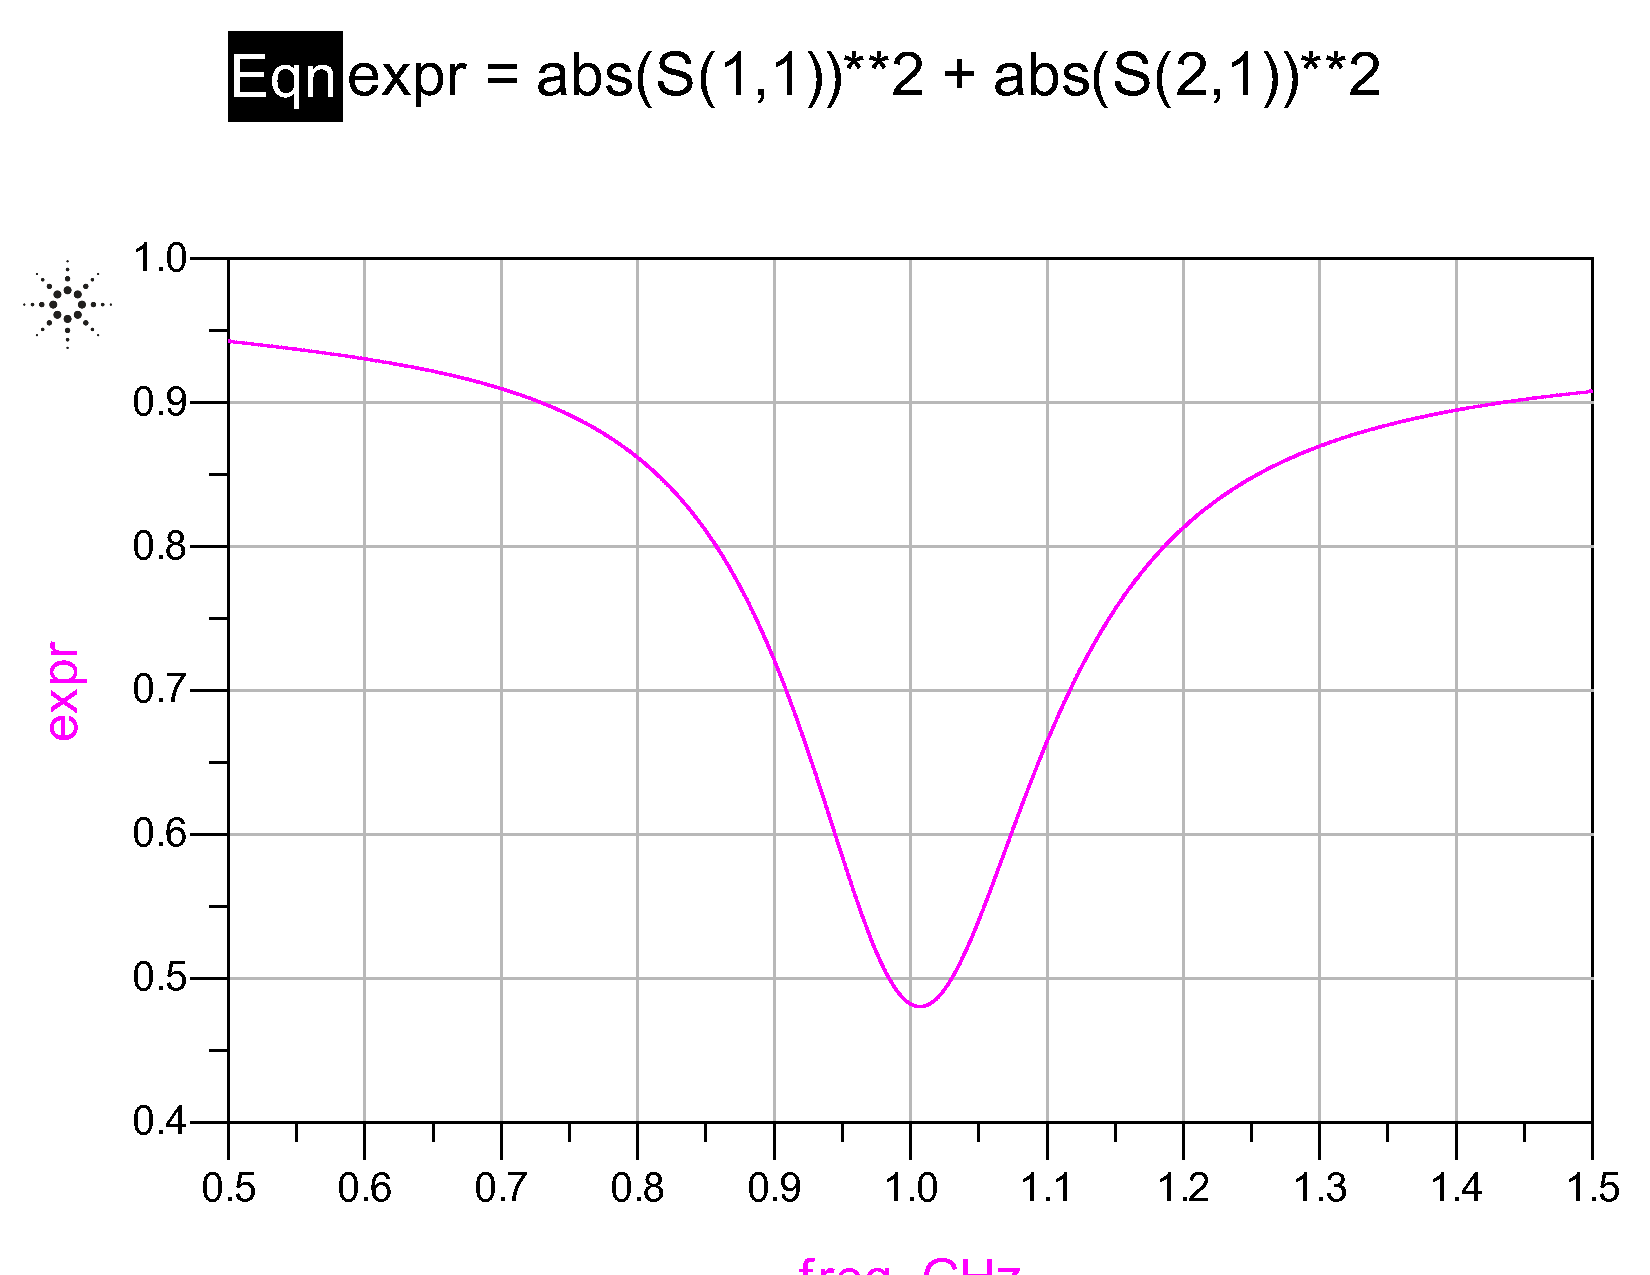
\includegraphics[width=\textwidth-4cm]{problem3a_relationship.pdf}
    \end{figure}
    In the finite Q simulation, the relationship $|S_{11}|^2 + |S_{21}|^2 = 1$ doesn't hold near the center frequency. This is due to the internal loss of the finite Q components.

    \item {\color{blue}Design a matching network between a $1000 \Omega$ load impedance and a $50\Omega$ source impedance at 1 Ghz. The inductor and capacitor quality factors are 20. The design goal is to achieve the lowest insertion loss. Calculate the insertion loss and verify your design using ADS.}

    \begin{align*}
        \text{IL} = \frac{1}{1 + \frac{N}{Q_u} \sqrt{(\frac{R_{hi}}{R_{lo}})^{1/N} - 1}}
    \end{align*}

    We use this equation with our design variables to find the ideal value of $N$. We let $Q_u = Q_{cap} || Q_{ind} = 10$.

    \begin{figure}[H]
        \centering 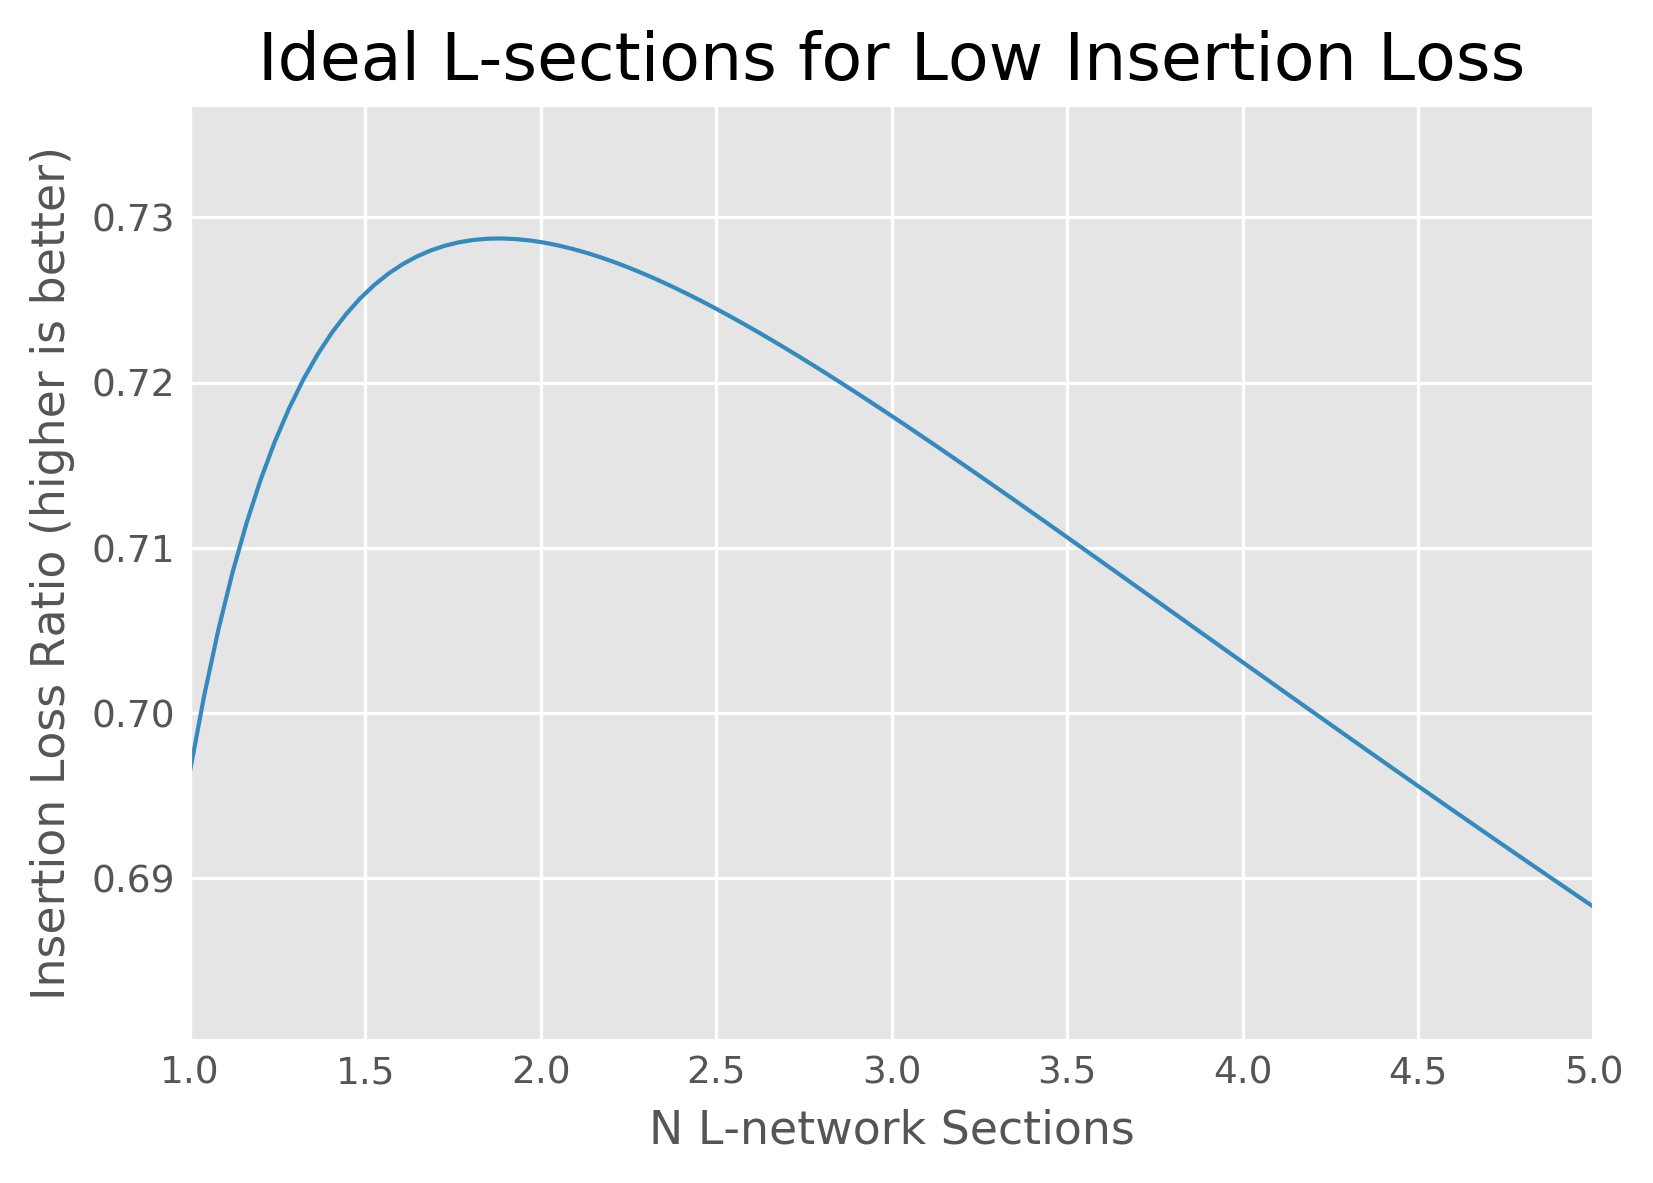
\includegraphics[width=\textwidth-4cm]{problem3b_ideal_sections.png}
    \end{figure}

    Insertion loss is minimized with 2 L-network stages. $IL_{max} = 0.729$.

    \begin{align*}
        R_{i,opt} &= \sqrt{R_L R_S} = 223.6 \\
        Q_{i,opt} &= \sqrt{(\frac{R_{hi}}{R_{lo}})^{1/N} - 1} = 1.863
    \end{align*}

    Now we can again go through the process of calculating actual component values.
    \begin{center}
    \begin{tabular}{l | l | l |}
        & L-network 1 & L-network 2 \\ \hline
        $X_p$ & 536.66 & 120.0 \\ \hline
        $X_s$ & 416.66 & 93.168 \\ \hline
        $C$ & 0.296 pF & 1.326 pF \\ \hline
        $L$ & 66.3 nH & 14.8 nH \\ \hline
    \end{tabular}
    \end{center}

    Again assuming that capacitors are in shunt and inductors in series. Use these values and run a finite Q simulation.
    \begin{figure}[H]
        \centering 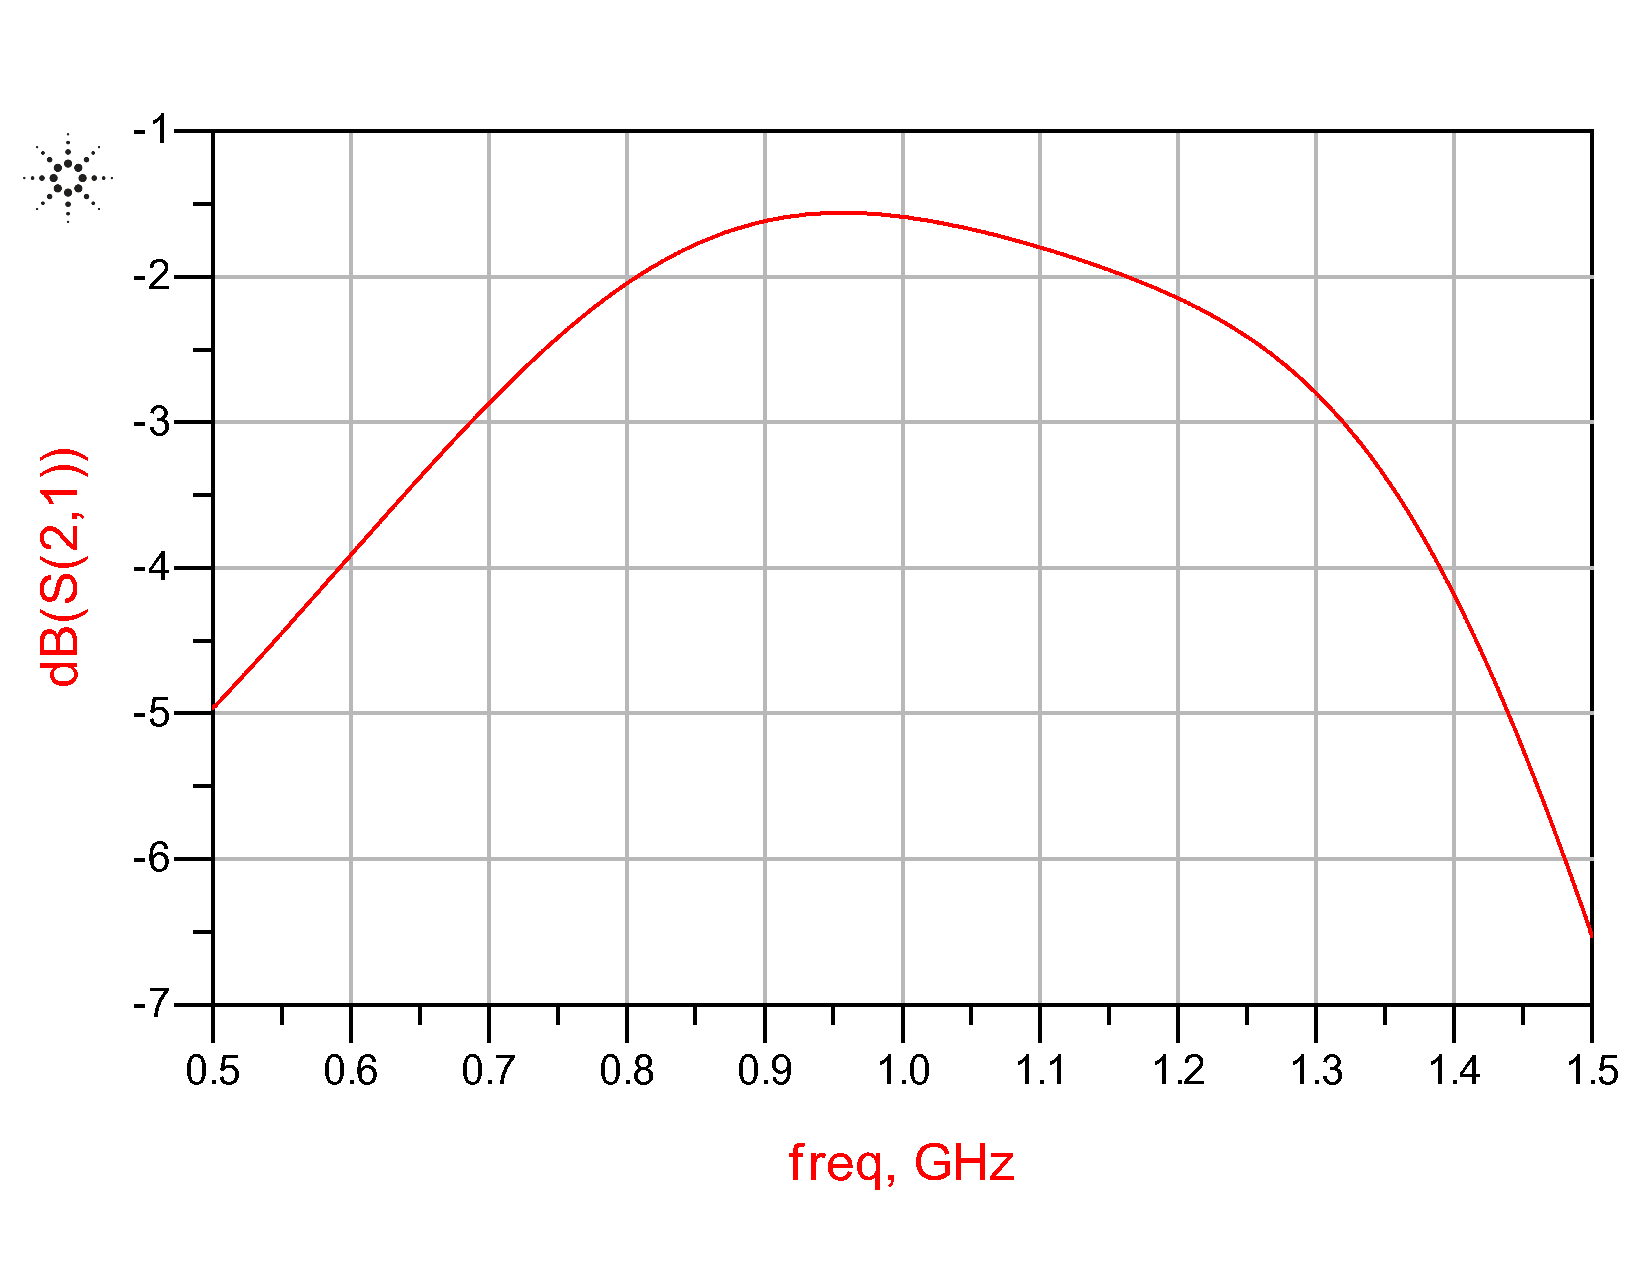
\includegraphics[width=\textwidth-4cm]{problem3b_insertion_loss.pdf}
    \end{figure}

    The simulation confirms a low insertion loss of around -1.5 dB. This is about 4dB better than the $\Pi$ network.
\end{enumerate}

\end{document}
